\documentclass[conference]{IEEEtran}
\IEEEoverridecommandlockouts
% The preceding line is only needed to identify funding in the first footnote. If that is unneeded, please comment it out.
\usepackage{cite}
\usepackage{amsmath,amssymb,amsfonts}
\usepackage{multicol}
\usepackage{algorithmic}
\usepackage{graphicx}
\usepackage{textcomp}
\def\BibTeX{{\rm B\kern-.05em{\sc i\kern-.025em b}\kern-.08em
    T\kern-.1667em\lower.7ex\hbox{E}\kern-.125emX}}
\begin{document}

\title{Thread Pool in GeckoDB/BOLSTER - Integrating a Thread Pool into a high performance Database System \\
}

\author{
	\IEEEauthorblockN{Robert Jendersie, Johannes Wuensche, Johann Wagner, Marten Wallewein-Eising}
	\IEEEauthorblockA{\textit{Otto-von-Guericke University} \\
		Magdeburg, Germany \\
		\emph{firstname}.\emph{lastname}@st.ovgu.de} \and
}

\maketitle

\begin{abstract}
Processing tasks in parallel is used in nearly all applications to keep up with the requirements on modern software systems. However, the implementation of parallel processing can differ strongly depending on the desired use cases and reach from spawning dozens of threads to reuse threads in thread pools. In this paper, we show an implementation of a thread pool to process independent tasks in parallel including the waiting for a set of processed tasks. We also compare the thread pool implementation against a baseline, which spawns new threads for parallel data processing. The evaluation of the thread pool shows, that designing and implementing a thread pool is a balancing act between generalization of tasks and the processing performance. Additionally, we show that the task and thread pool configuration depending on the use case has a high impact on the thread pool performance.
\end{abstract}

\begin{IEEEkeywords}
Thread Pool, GeckoDB, BOLSTER
\end{IEEEkeywords}

\section{Introduction}
Since the amount of data that is stored and processed by modern database systems is growing fast, sequential data processing as only possibility is inconceivable. Applications have to process data in parallel to reach sufficient throughput to fulfil appropriate requirements. 

Parallel data processing can be achieved by different approaches, like instruction and data parallelism or multi threading. In this paper, we focus on multi threading by implementing a thread pool for the graph database system GeckoDB. The thread pool will be integrated into BOLSTER, a high performance library for parallel execution of primitives like for or filter on large data sets. In the current implementation, BOLSTER creates a fix number of threads for each call of a primitive. This approach is called \emph{thread-per-request}. Since many primitives are executed at the same time, many drawbacks arise from this implementation. 
First of all, the creation of threads comes along with overhead like stack initialisation and memory allocation. Secondly, creating a huge number of threads simultaneously may lead to large context switch overhead of the scheduler. Additionally, debugging and profiling applications that create many threads during runtime is 	time-consuming.

To overcome these drawbacks, we integrate an optimised thread pool in BOLSTER. Along with the implementation, we measure the performance of the primitives to determine the thread pool overhead. Additionally, we measure metrics like \emph{idle and job time} of threads to evaluate correct thread pool sizes for the considered use cases.  In this work we make the following contributions:
\begin{itemize}
	\item We describe our design and implementation of the thread pool 
	\item We evaluate the possibility to wait for a group of task in the calling thread
	\item We compare our thread pool against the existing implementation in BOLSTER
\end{itemize}
We organized the rest of the paper as follows. In Section 2, we give preliminaries about the considered task configuration and about thread safe access of memory. In Section 3, we show our design and implementation of the thread pool and examine our experimental environment in Section 4. In Section 5, we describe the results of our performance evaluation. In Section 6, we name related work and state our conclusion and future work in Section 7.

\section{Preliminaries}
In this section, we define our configuration of tasks that are processed by the thread pool and state difficulties of synchronizing thread access to memory.

\begin{figure*}[htbp]
	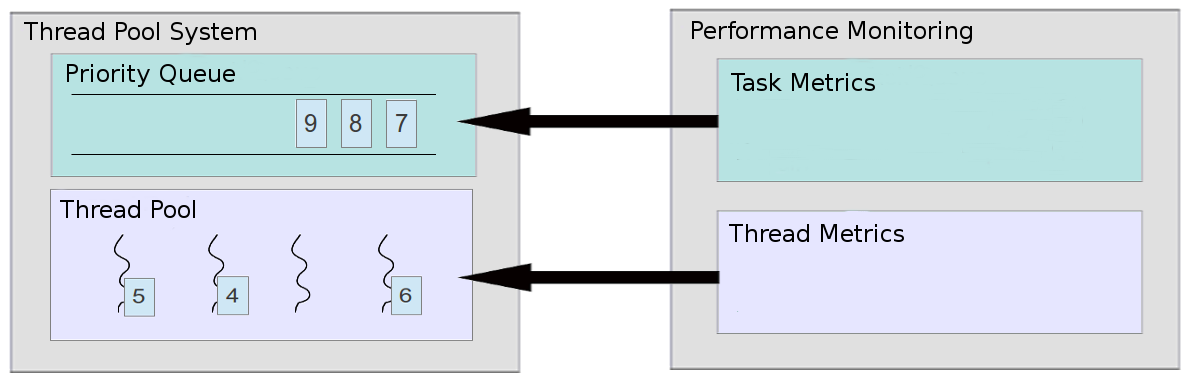
\includegraphics[width=1.0\textwidth]{img/pool_structure.png}
	\caption{Design of the thread pool system}
	\label{fig0}
\end{figure*}

\subsection{Task Configuration}
We define a Task as a structure containing data that has to be processed and an operation that has to be executed on the data. In this work, we define tasks as \emph{independent}, which means tasks do not have dependencies on other tasks and can be processed independently. Furthermore, we expect the data passed to two tasks are stored in different memory locations. Consequently, while executing the task operation, threads do not access the same memory locations. 

Each task can be enqueued with a priority. The priority zero is the highest and the task will be processed by the next free thread. The higher the priority of the task is, the further it is placed behind in the queue. Additionally, we only consider not preemtable tasks. Once a task is assigned to a thread, the thread will finish the operation of the task before getting a new one. 

\subsection{Synchronizing Memory Access from Threads}
Parallelism with multi threading works great as long as each thread works on a separate memory area. During task scheduling, the scheduler has to know the state each thread has. This can be solved with signal handling or by writing the current thread state into main memory. In this work, we implement the second approach to avoid having another thread that only schedules tasks to other threads. 

Threadsafe access to memory can be achieved by different approaches. Firstly, a mutex thread can manage the access for multiple other threads. Secondly, atomic operations ensure the safe access from different threads to the same memory. We use both approaches for different parts of the thread pool. Since using a mutex thread can decrease access performance, we decided to execute atomic operations on the memory containing the thread state informations. For example, the function \emph{atomic\_compare\_exchange\_strong} performs a compare and, if the result is true, an exchange of the memory in one atomic operation. We use a mutex thread to synchronize the enqueueing of tasks into the priority queue.

\section{Implementation}
In this section, we describe in detail the design and implementation of our thread pool. We show how tasks are enqueued regarding their priority and how the waiting for tasks is implemented. Additionally, we state our thread metrics and how they are integrated in the thread pool design. 

\subsection{Architecture of the Thread Pool}
Compared to simply create threads on demand, managing threads in a pool comes along with memory and CPU overhead. The thread pool must know information about the state each thread has and his assigned task. To measure metrics of threads and tasks, additional memory for threads and tasks is required. 

In Figure 1, we show our design of the whole thread pool system, containing the thread pool itself, the task priority queue and the performance monitoring. Since measuring performance metrics lead to memory and CPU overhead, we decided to exclude the performance measurements from the thread pool to make it optional. The performance monitoring can be activated as a boolean parameter to the thread pool create functions. Consequently, in the target database system, the designers can decide for each thread pool instance, if performance monitoring should be applied. 

The thread pool system includes an array of threads and a priority queue to store the passed tasks. We decided to implement the thread pool using the POSIX thread library to provide the thread pool for multiple operation systems like Linux and Unix. Additionally, we avoid using custom compiler flags to ensure that the thread pool can be compiled with different compilers. The thread pool itself contains a variable number of threads. Since Xu et al. \cite{xu2004performance} and Ling et al. \cite{ling2000analysis} show the importance of accurate thread pool size, we add a resizing function for our thread pool, which enables to change the amount of threads at runtime.

\subsection{Thread Pool and Task Queue}
Threads and tasks are two major entities in the thread pool system. As we can observe from Figure 1, thread pool and task queue are two data structures used to store the required information related to the threads and the submitted tasks, respectively. Each spawned thread can be either working on a task or waiting for the next task. Consequently, we define the states of a thread as \emph{busy} and \emph{waiting}. A busy thread changes to waiting after processing its task if no other task is enqueued. Waiting tasks do busy waiting until there are new tasks available.

Each assigned task contains a function pointer to a routine and a pointer to data. We implemented the task queue as a generic priority queue that uses a mutex thread to enqueue tasks threadsafe. Every time a new task is enqueued to the task queue, two scenarios can occur. If the new task has a priority, it is placed in the right slot of the task queue regarding its priority and the subsequent tasks are relocated. If the  new task has no priority, it is appended to the end of the queue. Furthermore, tasks can refer to a handle, which is used by the thread pool to wait for a specific amount of tasks.
\begin{table*}[htbp]
	\caption{Functions provided by the thread pool to process tasks}
	\begin{center}
		\begin{tabular}{ c c }
			\hline
			\textbf{Function Name}&\textbf{Explanation}\\
			\hline
			thread\_pool\_enqueue\_task & Enqueue task with optional handle \\
			thread\_pool\_enqueue\_tasks & Enqueue tasks with optional handle \\
			thread\_pool\_wait\_for\_task & Waits until the tasks referenced by the handle are completed. \\
			thread\_pool\_enqueue\_tasks\_wait & Enqueue tasks and wait until they are finished. The main thread also participates in task execution\\ 
			thread\_pool\_wait\_for\_all & Wait until all enqueued tasks are finished. The main thread also participates in task execution \\ \hline
		\end{tabular}
		\label{tab1}
	\end{center}
\end{table*}
\subsection{Processing Tasks}
Processing tasks in a thread pool is a balancing act between generalization the of tasks and the performance of their execution. Therefore, we provide a set of functions to process task in the thread pool to match different requirements of BOLSTER. In Table 1, we show the functions provided by our thread pool to process tasks. One of the requirements of BOLSTER is waiting until a set of tasks is finished. To achieve the same performance as the baseline implementation reaches, we let the main thread first participate in the execution of the tasks and then wait until all tasks with the same handle are finished. 

To show the processing of tasks, we consider the function \emph{thread\_pool\_enqueue\_tasks\_wait}. In Figure 2, we show the flow of task enqueueing and execution in the thread pool system using this function. In the first step, tasks are passed as a parameter to the enqueue function provided by the thread pool. The tasks have to be created before passing and later on freed after processing by the calling function.  We provide different functions to enqueue a single task or an array of tasks. 

In the next step, the tasks will be enqueued into the priority queue of the thread pool. Before enqueueing, the function \emph{thread\_pool\_enqueue\_tasks\_wait} creates a handle and links all tasks to it. After enqueueing the tasks to the priority queue, the waiting threads in the thread pool pop the enqueued tasks from the priority queue and execute the routine of the task. This happens asynchronously to the calling function and therefore is not considered as an own step of the process. The calling threads gets one of the passed tasks and processes it. After finishing the task, the calling thread waits until all other tasks referring to the created handle are finished and then returns to the calling function. In the next section, we show the waiting for tasks with handles in detail.

\begin{figure}
	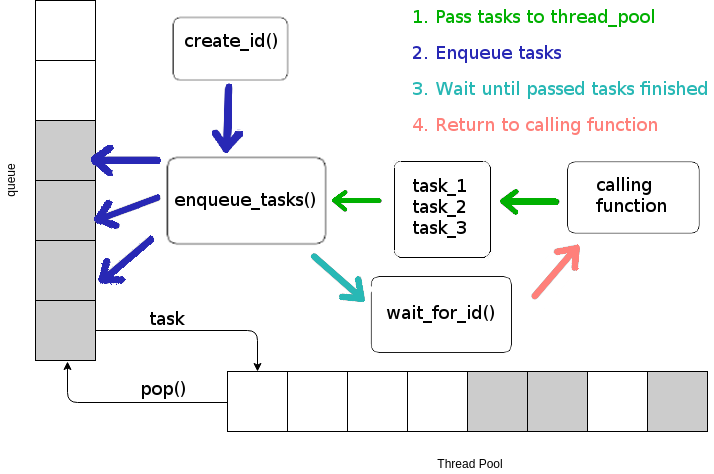
\includegraphics[width=0.5\textwidth]{img/pool_queue.png}
	\caption{Workflow of task enqueueing and execution in the thread pool}
	\label{fig1}
\end{figure}

\subsection{Waiting for Tasks}
As mentioned before, the thread pool provides the functionality to let the calling function participate in the task execution and wait until all passed tasks are processed. To wait for a set of tasks, it is not sufficient to look firstly in the priority queue for the tasks and then in the state of the thread pool, since popping tasks out of the queue is not an atomic operation. Consequently, tasks can have a state between being enqueued in the queue and being executed by a thread. 

To solve this problem, we implement the waiting for a set of tasks using a slotmap. In Figure 3, we show the concept of our slotmap. During the enqueueing process of tasks, a set of tasks are referred to a slot in the slotmap. Each slot contains a number of open tasks to be finished and a generation counter. We name the number of open task \emph{openTaskCount} and the generation counter \emph{genCount}. Every time a set of tasks is enqueued, a slot with $openTaskCount = 0$ is selected and the \emph{genCount} increases. Every time a thread finishes a task, the $openTaskCount$ of the referred slot is decreased. As mentioned before, multiple tasks can refer to a single handle. This handle also refers to a slot and has additionally assigned a generation value. The waiting algorithm loops over the following conditions before returning to the calling function: It checks if the number of open tasks is zero or if the generation counter of this slot has changed. If one of these conditions is true, the waiting algorithm returns to the calling function.

To clarify the procedure of the waiting algorithm, we consider the second slot in Figure 3. The tasks $10, 12, $ and $13$ as well has the first handle refer to this slot. Consequently, these tasks were enqueued referring to the first handle. Before any of the three tasks is processed, the slot has the following state: $openTaskCount = 3$ and $genCount =  2$. Since the waiting thread does not know when tasks are executed due to the asynchronous behaviour, the waiting algorithm starts looping as long as the following condition is true: $openTaskCount \neq 0$ \&\& $genCount = 2$. For each finished task, $openTaskCount$ is decreased. It is not sufficient to check only $openTaskCount \neq 0$, since the slot can be reused before the waiting algorithms noticed that $openTaskCount = 0$. Consequently, we check if the slot stays on the same generation. If the slot is reused, $genCount$ increases and the second part of the condition returns false.

\begin{figure}
	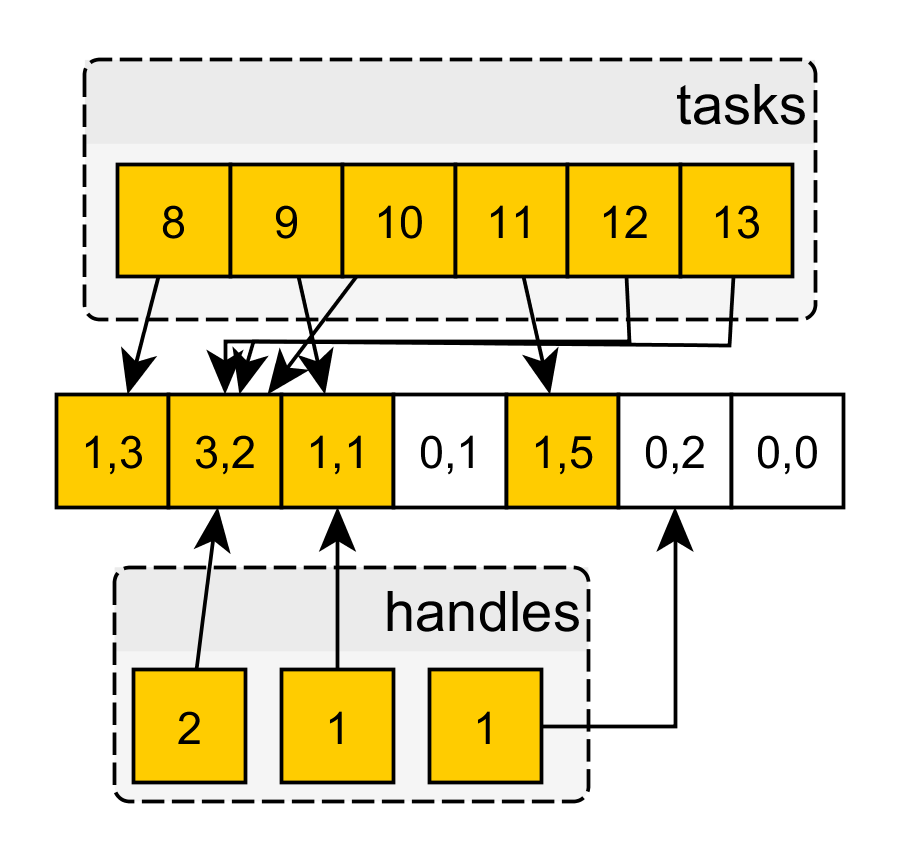
\includegraphics[width=0.4\textwidth]{img/waitingconcept.png}
	\caption{Concept of waiting for tasks using a slotmap}
	\label{fig2}
\end{figure}

\subsection{Managing Thread States}
As mentioned before, accessing the same memory location from different thread may lead to race conditions, which means the program behaviour depends on the accessing order of the threads. For example, while one thread updates data at a specific memory location another threads writes into the data, which results to inconsistency. In Section 2, we presented two approaches to handle multithreaded access to the same memory location, mutex threads and atomic operations and we state where those approaches are used in our implementation. In this subsection, we focus on atomic operations to manage thread states. We consider the following steps for a thread to update its state. At first, the current state has to be checked and, depending on the current state, the state has to be updated. If these steps are implemented using an if statement and an update function, the complete update procedure is not atomic. Consequently, another thread can update the state between the check of the current state and the update. To avoid this, we use the function \emph{atomic\_compare\_exchange\_strong} \cite{atomicstrong} of the stdatomic lib. This function combines the check and update in one atomic procedure. We implemented every thread state access with this function to ensure atomic thread state updates. After presenting the enqueueing, processing, and waiting for tasks, we show the second component of our thread pool, the performance monitoring.

\subsection{Performance monitoring}
The performance monitoring component of the thread pool system is responsible for collecting data about threads, tasks, and the whole thread pool system. We will use the information collected in this component for analysis and performance optimization in later stages. As mentioned before, the performance monitoring is an optional component, since evaluating the following statistics can reduce the execution performance of our thread pool. We divide the collected statistics into the sections \emph{task statistics}, \emph{thread statistics}, and \emph{thread pool statistics}.

\subsubsection{Task Statistics}
Collecting statistics about the time tasks spend in the priority queue or during the execution is useful to tune the thread pool configuration for better performance results. In Table \ref{tab2} we show the statistics that are collected for each task. 

\begin{table}[htbp]
	\caption{Task statistics with their internal names and descriptions}
	\begin{center}
		\begin{tabular}{ c c }
			\hline
			\textbf{Statistic name}&\textbf{Description}\\
			\hline
			enqueue\_time & Time when the task was enqueued \\
			execution\_time & Time when the task execution begins \\
			complete\_time & Time when the task execution is finished \\
			\hline
		\end{tabular}
		\label{tab2}
	\end{center}
\end{table}

How long a task waits in the queue before being executed is a good metric to adjust task priority or the thread pool size. For example, if an enqueued task with priority 0 still has a large difference between \emph{enqueue\_time} and \emph{execution\_time}, the thread pool size may be too small. Otherwise, if a large number of tasks without high priority have small differences between \emph{enqueue\_time} and \emph{execution\_time}, this may indicate that the thread pool size is too large. A better indicator of not optimized thread pool sizes are statistics per thread.

\subsubsection{Thread Statistics}
As mentioned before, adjusting the thread pool size based on task statistics may not be very precise. Consequently, collecting statistics per thread is necessary for a good evaluation of the relation between tasks and threads. In Table \ref{tab3}, we show our statistics collected for each thread in a thread pool instance. 

\begin{table}[htbp]
	\caption{Thread statistics with their internal names and descriptions}
	\begin{center}
		\begin{tabular}{ c c }
			\hline
			\textbf{Statistic name}&\textbf{Description}\\
			\hline
			waiting\_time & Time the thread spend waiting (ms) \\
			busy\_time & Time the thread spend executing tasks (ms)\\
			task\_count & Number of tasks the thread has executed \\
			\hline
		\end{tabular}
		\label{tab3}
	\end{center}
\end{table}

The \emph{busy\_time} of a thread strongly depends on the executed tasks and therefor is a metric that gives less information about the thread pool itself. In contrast, the \emph{waiting\_time} is a good indicator to reveal less used threads in the thread pool to determine an optimal amount of threads for the current use case. Furthermore, the \emph{task\_count} of thread compared to the number of tasks processed by the thread pool indicates the degree of usage of the thread. To give further possibilities for optimizing the thread pool, we collect statistics for each thread pool instance.

\subsubsection{Thread Pool Statistics}
To consider the thread pool instance, an important metric is the average waiting time of tasks. In order to optimize the thread pool size, a balanced relation between the waiting time of tasks and the number of threads must be found. Furthermore, at a specific time, the relation between enqueued and completed tasks can be interesting. In Table \ref{tab4}, we show our statistics collected for each thread pool instance.

\begin{table}[htbp]
	\caption{Thread pool statistics with their internal names and descriptions}
	\begin{center}
		\begin{tabular}{ c c }
			\hline
			\textbf{Statistic name}&\textbf{Description}\\
			\hline
			working\_time & Time the thread pool runs (ms) \\
			task\_complete\_count & Number of tasks the thread pool has completed\\
			task\_enqueued\_count & Number of tasks the thread pool has enqueued \\
			avg\_complete\_time & Average time span from enqueueing until \\
			& execution of tasks \\
			avg\_wait\_time & Average time of tasks spend in the queue \\
			\hline
		\end{tabular}
		\label{tab4}
	\end{center}
\end{table}

We will use these statistics to adapt our thread pool implementation to different use cases later on. In the next sections, we define our experimental environment, the implementation of our tests including the measured metrics and the test results.

\section{Experimental Environment}	
In this section, we present our experimental environment focussing on the design of our benchmarks and the system configuration we used to evaluate our thread pool implementation.

\subsection{Evaluation Setup}
In our evaluation setup, we focus primarily on the comparison of using our thread pool against the baseline implementation of creating new threads at runtime of BOLSTER. We simulate calls of BOLSTER primitives with different thread pool and task configurations and compare the results against the baseline. 

Additionally, we evaluate the metrics for threads, tasks and the thread pool mentioned in Section 3.F regarding the thread pool and task configuration used in the BOLSTER primitives. To evaluate optimal configurations for the thread pool, we consider the relation between idle and busy time of the thread pool and the average waiting time of tasks.

Furthermore, we compare the scope and usage of our thread pool against an existing implementation \emph{Threading Building Blocks (Intel TBB)} \textbf{TODO: cite!} written in C++. Since Intel TBB uses completely different approaches to parallel the execution of tasks, a direct performance comparison may not lead to reliable results. Therefore, we evaluate the usage and the scope both implementations give.
 
\subsection{Experimental Configuration}
\textbf{TODO: Change?}\\The operating system is Ubuntu 17.04 with linux kernel version 4.13 running in a virtual machine on an Intel Core i7-6700HQ, 4x 2.6 GHz (Skylake) and 8GB DDR3 RAM running on 1600Mhz. We reduce the number of cores of the virtual machine to 4 instead of 8 virtual cores of the CPU. The CPU has 256KB L1 cache, 1MB L2 cache, and 6MB L3 cache. All simulations are repeated three times and a median value of all repetitions is used for evaluation. 	

\section{Evaluation}

\section{Related Work}

\section{Conclusion and Future Work}

\bibliographystyle{splncs}
\bibliography{paper_thread_pool} 

\end{document}
